\chapter{Method}

The aim of this project was to investigate the possibility of creating hardware accelerator for a machine learning algorithm. Sadly, creating a module that provides the full functionality of a CNN requires more time than what was available for this project. But we were able to realize part of the network, the convolution and the subsampling/pooling layer. This chapter will describe the design and the reasoning behind it. 

\section{Potential for parallism}

A vast amount of the computation required by a CNN can be done in parallel, something that is illustrated by the fact that GPU implementations executes faster than a CPU by several factors. So, in order to accelerate the processing of the network it is important that these potential parallelizations are identified and exploited. The most obvious being:

\begin{enumerate}
	\item The computation of each of the invidual feature maps.
	\item The subsampling/pooling of each of the feature maps. 
	\item The activation of each neuron in the fully connected layer. 	
\end{enumerate}

Some of less obvious ones are within the mentioned parallelizaitions themselves. The convolution of a matrix $ n \times n $ using a $ k \times k $ kernel consists of $ n - k + 1 $ convolution operation, which each can be done in parallel. Thus convoluting the whole matrix could potentially take only the time it takes to perform one convolution operation, by doing all the operations in parallel. The subsampling/pooling operation can also be parallelized by pooling all of the submatrices at the same time.  
	
The activation of each neuron by itself is a bit harder to parallelize, since its basically a set of  \textit{n} multiply and accumulate operations. One option is to parallelize them by doing them in a binary-tree-like structure, which will reduce the time it takes from \textit{n} time to $ log_2 n $ time. But considering that vast amount of neuron activations that is to be computed, it might not be worth the increased complexity of the hardware accelerator. Unless you have unlimited hardware resources. 



\section{Hardware}

In this project we had a Spartan 6 LX16 development board at our disposal, something which provided us with 32 \textit{digital signal processors} (DSP). Since convolution is basically a series of multiply and accumulate (MAC), the DSPs are essential to accelerate the operation. Ideally, we would have several times as many DSPs in order to fully utilize the potential parallelism of the network.  

\section{Architecture}


For simplicity we will refer to both the layer performing convolution and the layer performing subsampling/max-pooling as the convolution layer. 

\subsection {Convolution layer}

The convolution layer takes \textit{n} images as input, $ I_1, I_2, \dots, I_n $, and produces \textit{m} intermediate outputs, $O_1, O_2, \dots, O_m $. It also contains \textit{m} kernels, $ K_1, K_2, \dots, K_m $. Each kernel $ K_i $ is convolved with all the input images, and each respective pixel from each convolution is then summed, added a bias to, and sent through a non-linear function. Afterwards the resulting matrix is subsampled/max-pooled, where it is divided into $ p \times p $ non-overlapping neighborhoods, from which the maximum value is extracted. The result of the max-pool operation the output image $ O_i $. 
 


\begin{figure}[h!]
  \centering
      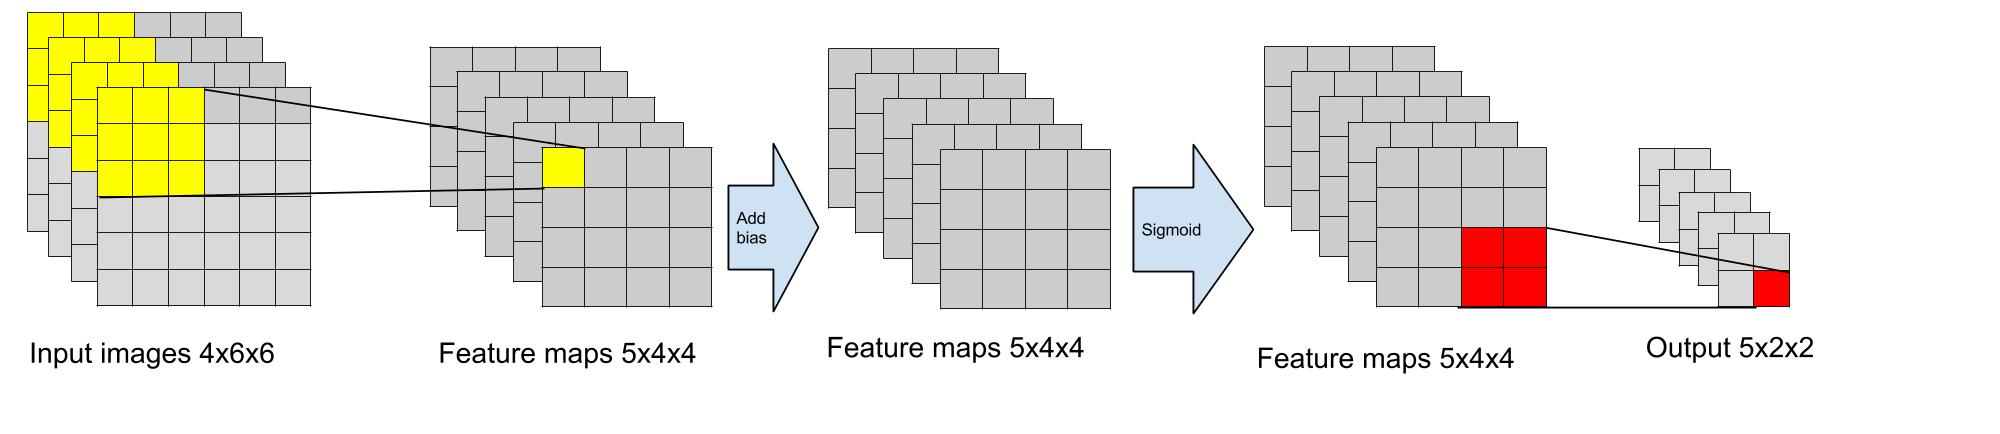
\includegraphics[width=1.0\textwidth]{Figures/Method/Convolution_subsample_pool}
  \caption{A visual overview of the operations performed by the convolution layer. Yellow represents the convolution operation, and red represents the subsampling/max-pooling operation. Note that all the input images is used to produce a single entry in the feature map.}
\end{figure}



The overall architecture of the convolution layer is separated into five modules:

\begin{itemize}
	\item \textbf{The convoluter}, performs the convolution operation on the input.
	\item \textbf{The intermediate feature map buffer}. Since the resulting feature map is the sum of the convolutions of all the input images, this buffer is needed to store the results from the previous convolution, so that it can be added to the current convolution. In the first layer of the network there is only one input image (i.e. $ n = 1 $), thus no summation is needed.
	\item \textbf{Bias register}. Contains the bias value, and adds it to each convoluted pixel. 
	\item \textbf{Sigmoid}. Performs the non-linear function sigmoid on the feature maps.
	\item \textbf{Subsample/max-pooler}. Performs the subsample/max-pool operation on the feature maps. 
\end{itemize}

\begin{figure}[h!]
  \centering
      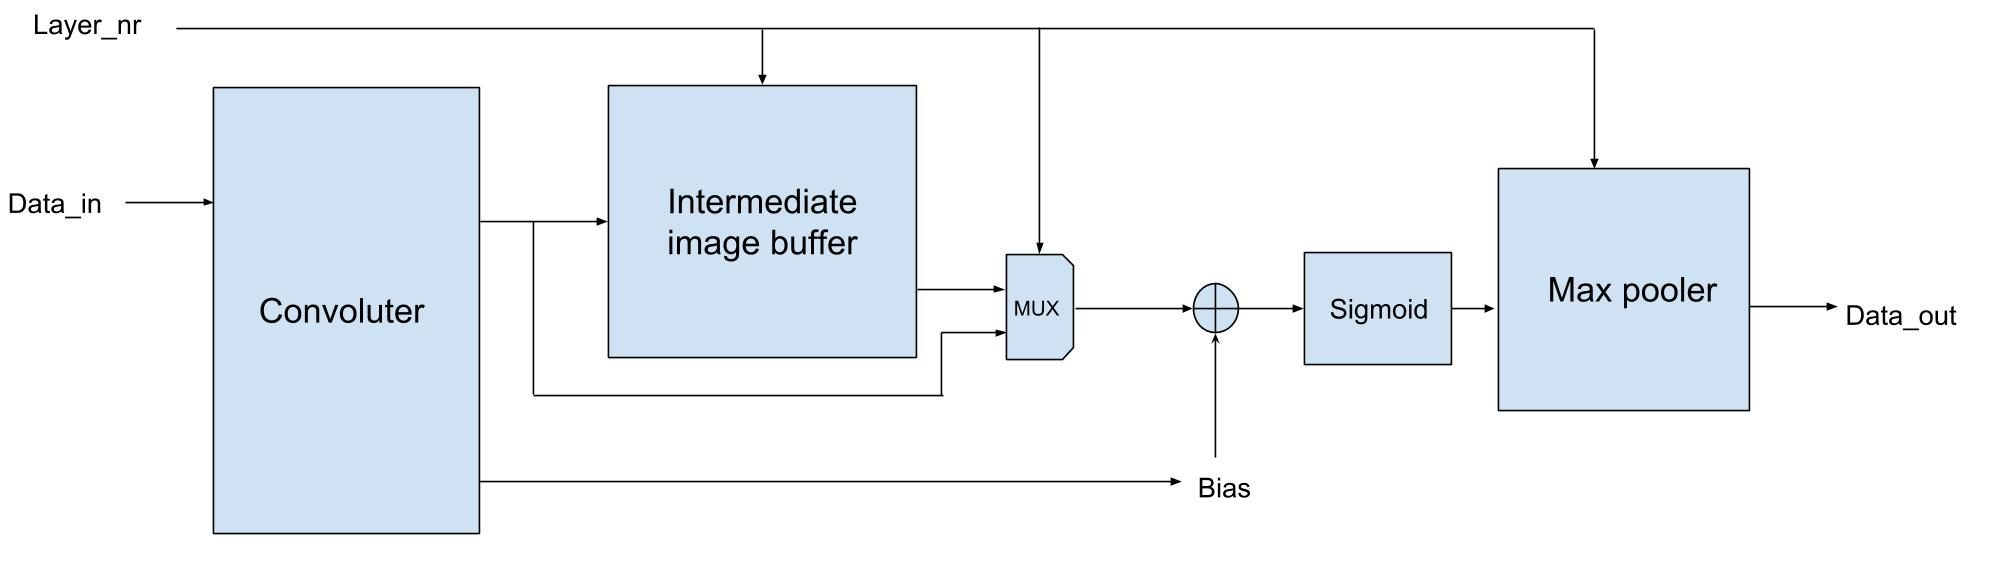
\includegraphics[width=1.0\textwidth]{Figures/Method/conv_layer_arch}
  \caption{The architecture of the convolution layer.}
\end{figure}


\paragraph{The convoluter} is inspired by \cite{Farabet2009}. The input is a $ n \times n $ image \textit{I}, and the output is a $ (n-k+1) \times (n-k+1) $ convolved image \textit{C}, using a $ k \times k $ kernel \textit{K}. Every clock cycle the module takes in a pixel as input, and after a certain delay it will output a processed pixel almost every cycle. Each pixel is inputted once, left to right, one row at a time. 

It consists of 2D grid of multiply and accumulate (MAC) units which represents the convolution kernel. Thus the grid dimension is equal to the kernel dimension. In every MAC unit there is a register that contains the respective kernel weight. In every clock cycle the MAC units multiply the input pixel with its weight, and then accumulates the result from the previous cycle of the MAC unit to the left. 

At the end of each row of MACs there is $ n - k $ shift registers. The result of the last MAC in each row is stored in the first shift register, and the first MAC in each row takes the value of the last shift register of the previous row as accumulation input. The exception being the absolute first and last MAC unit. Every clock cycle the values in the shift registers are shifted to the right. 

\begin{figure}[h!]
  \centering
      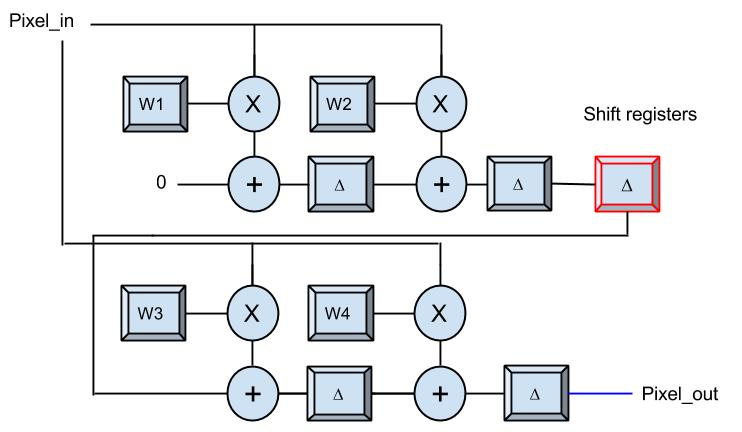
\includegraphics[width=1.0\textwidth]{Figures/Method/Convolver}
  \caption{The convolution module, when $ n = 3 $ and $ k = 2 $.}
\end{figure}
	
By providing this delay you only have to input each pixel once during the convolution. Generally every pixel is needed for $ k \times k $ convolution operations (the exception being the pixels close to the boarders of the image). Thus the shift registers are used to store the intermediate values of the convolutions until a pixel that is needed for the respective convolution operation is inputted. 

The delay these shift registers cause are the reason for the delay before valid output pixels are produced. Thus from when the convolution starts, the output will not be valid before $ k-1 $ rows of the image have been processed. And for every new image row, there will be a $ k-1 $ cycle delay before output is valid. This is demonstrated by the fact that the input image is a $ n \times n $ matrix, while the output matrix is a $ (n-k+1) \times (n-k+1) $ matrix. 

The loading of the weights takes $ k \times k $ clock cycles, and the processing of the image takes $ n \times n $ clock cycles. Thus the total number of cycles it takes to perform a full convolution of an image is $ n \times n + k \times k $. But \textit{n} tends to be larger than \textit{k}. e.g. $ n = 32 $ and $ k = 5 $ is a fairly normal problem size, which makes the weight loading take 25 clock cycles and the image processing 1024 cycles. This means that the execution time of the Convoluter is mostly primairly by the size of the image. It is important to note that the Convoluter is resource expensive, in that it requires $ k \times k $ DSP slices on the FPGA.

\begin{figure}[h!]
  \centering
      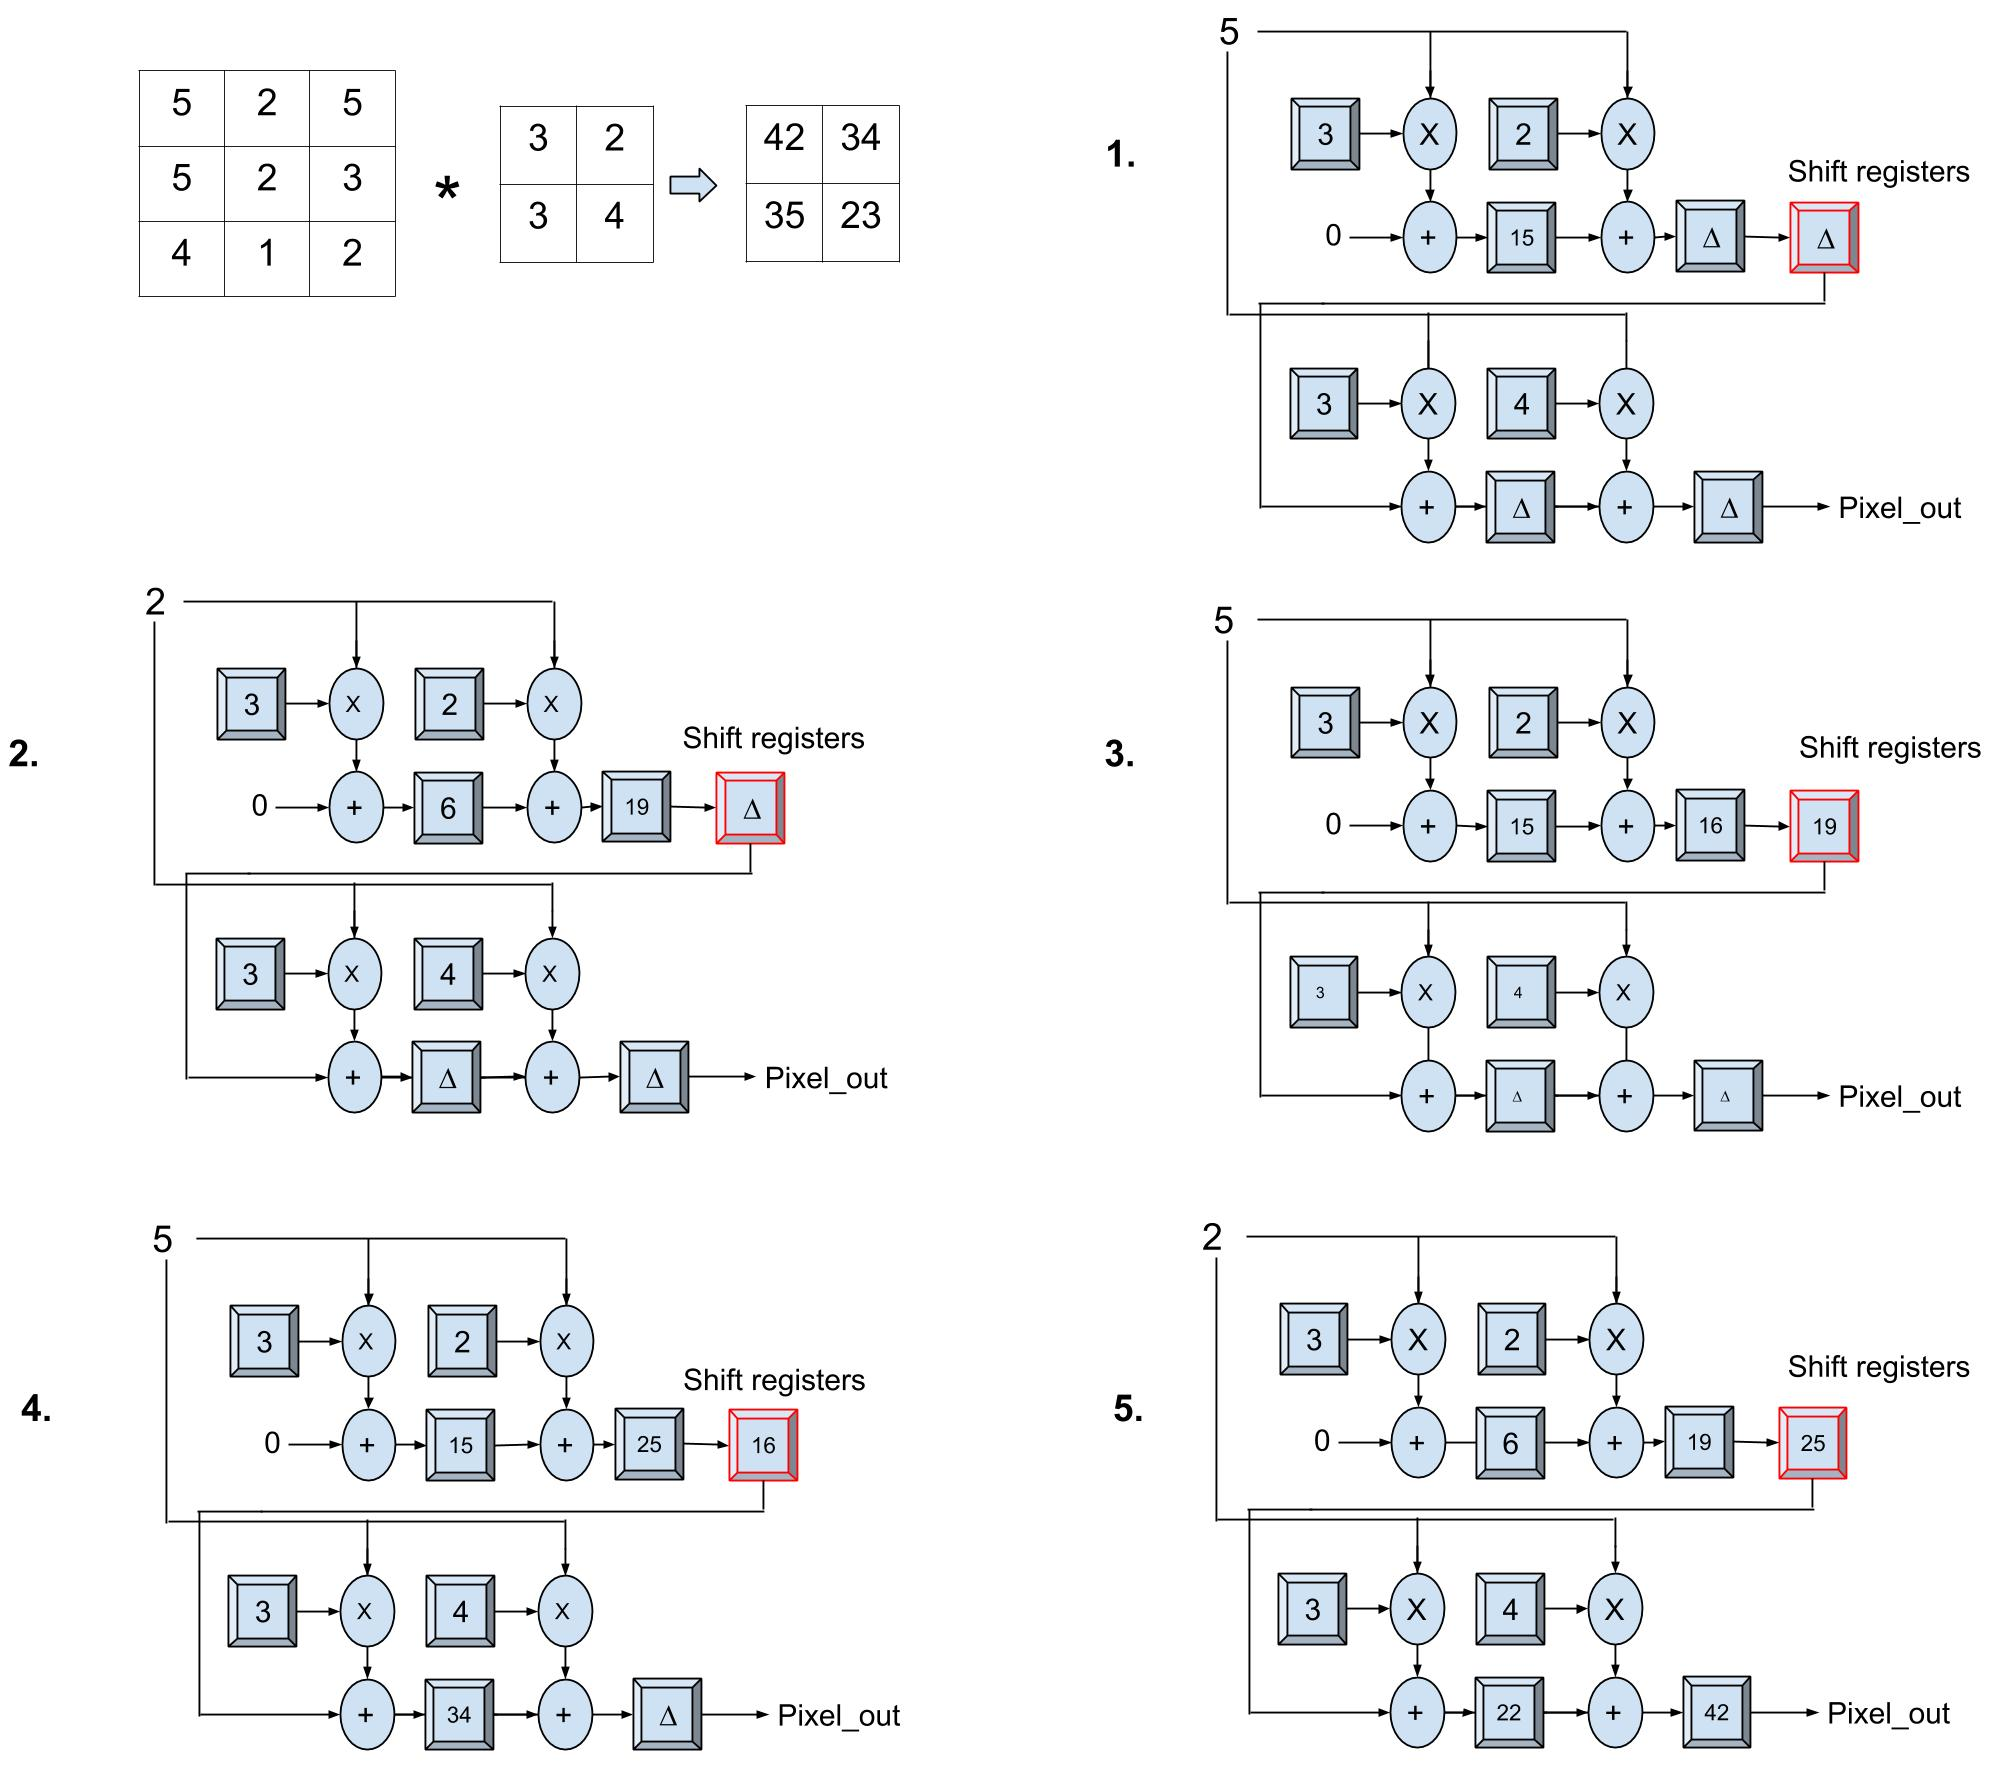
\includegraphics[width=1.0\textwidth]{Figures/Method/Conv_example}
  \caption{Example showing the five first clock cycle of an convolution. The weights of the kernel is already loaded into the MAC units, and every cycle a new pixel from the image in inputted. In the last example you can see that 42 is provided as the first output.}
\end{figure}

\vspace*{1\baselineskip}
REWRITE FIRST PART
\paragraph{The subsample/max-pooling module} (SS/MP) was designed to complement the CM and avoid being a bottleneck. Thus it was designed to act in the same streaming way as the convolution module, and be done processing at almost the same time. The input is a $ (n-k+1) \times (n-k+1) $ convolved image \textit{C}, and the output is a $ (n-k+1)/p \times (n-k+1)/p $ SS/MP image \textit{P}, where \textit{p} is the dimension of subsample neighborhood. As with the CM, one pixel is streamed in every cycle, and streamed out whenever a valid pixel is ready. Designed this way the SS/MP can process in parallel with the CM, by directly streaming the output of the CM into the SS/MP module. 

\begin{figure}[h!]
  \centering
      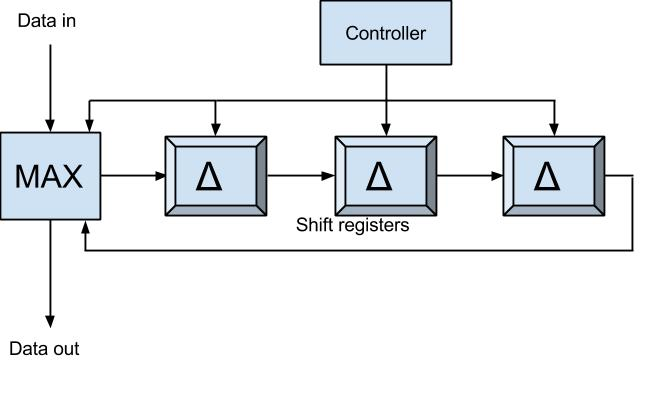
\includegraphics[width=0.5\textwidth]{Figures/Method/submax}
  \caption{Architecture of the subsampler/max-pooler.}
\end{figure}

The module compares the input with the current max value, and updates the max value accordingly. It contains a set of \textit{(n-k+1)/p} shift registers. Since the image is divided into $ p \times p $ non-overlapping neighborhoods, the module needs to store the current maximum value of previous neighborhood when a pixel from a new neighborhood is inputted. To do this the module contains two counters, \textit{row\_num} and \textit{column\_num}. When a new pixel is inputted the \textit{column\_num} counter is incremented, and when a new row is encountered the \textit{row\_num} counter is incremented. Every time $ column_num mod p = 0 $ the shift registers are shifted one to the right, and every time $ column_num mod p = 0 and row_num mod p = 0 $ a valid output is produced. 

The execution speed of the SS/MP module is bounded by the size of the input image, $ c \times c $ clock cycles, finishing one cycle after the last pixel has been inputted. 
Thus by streaming the output of the CM to the SS/MP, both will finish only a few cycles apart, effectively running both jobs in parallel. The resource usage of the module is bounded by the size of the subsampling dimension, since it requires a number of shift registers equal to the size of the dimension. But essentially its resource usage is quite low.  
